\chapter{Data Preparation}  \label{chapter:data-preparation}
As it is often the case with data science projects, the data preparation part is rather tedious. After the static and time series bond data has been extracted from Datastream -- which will likely take several days -- it is available in form of multiple data parts in Excel format. Since it is more convenient to perform further statistical analysis in a dedicated statistical environment, such as Stata or MatLab, the data needs to be brought into 'long' format, and additionally to be cleaned from null entries and outliers. The undertaken procedures are described in the following. 

\section{Data Formatting}  \label{section:data-formatting}
For the static bond data, there is not much to be done in terms of formatting. Its original format, as downloaded from Datastream, is mostly suitable for further analysis and can be directly imported into Stata. Stata is the statistical software utilized in the scope of this projects and fits well for most of the analysis tasks. 

The downloaded time series data is initially in 'wide' format and has multiple bonds in one row. It looks like shown in Fig. \ref{fig:original-excel-ts-data}. 

\begin{figure}[h]
	\centering
	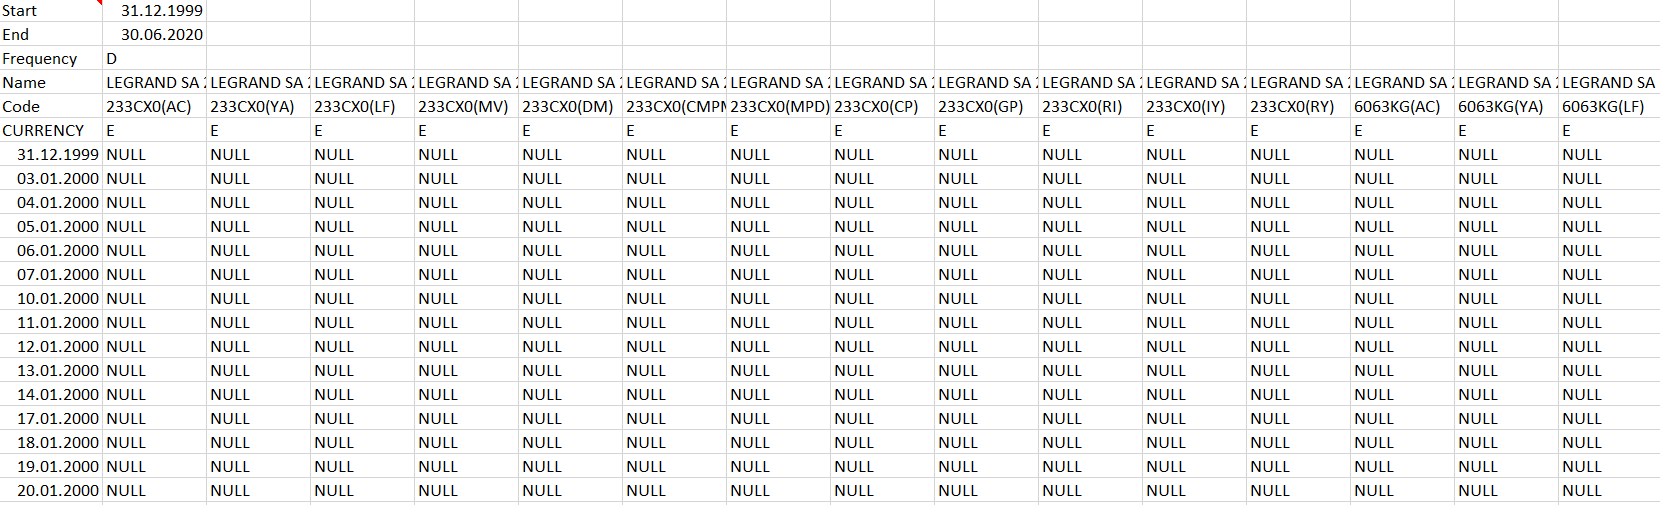
\includegraphics[width=1.0\linewidth]{figures/original-excel-ts-data}
	\caption{Sample of downloaded raw time series bond data}
	\label{fig:original-excel-ts-data}
\end{figure}

The goal is to transform this time series data into 'long' format, as can be seen in Fig. \ref{fig:long-format-excel-ts-data}, by saving the bonds one below the other. 
\begin{figure}[h]
	\centering
	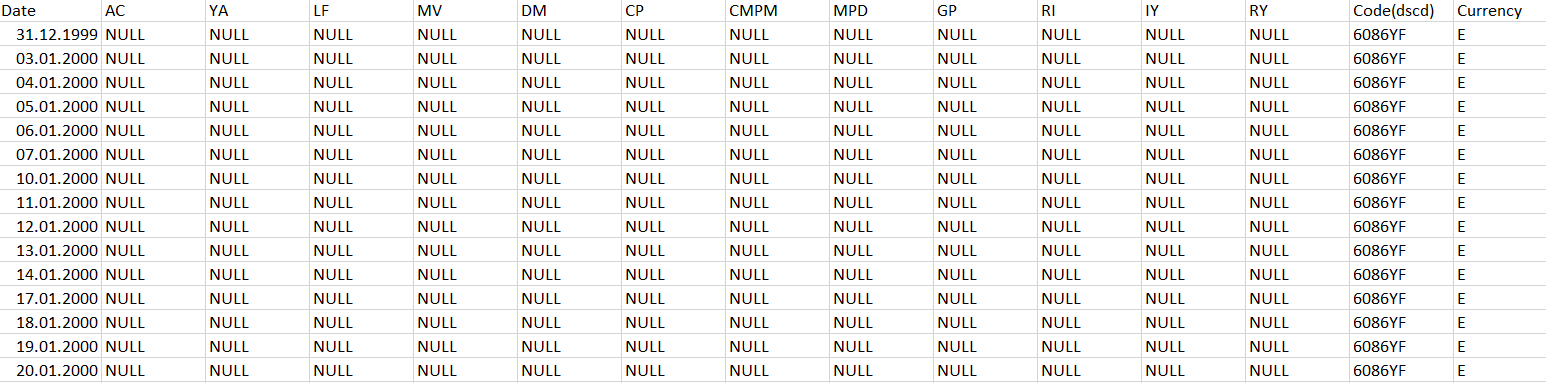
\includegraphics[width=1.0\linewidth]{figures/long-format-excel-ts-data}
	\caption{Sample of downloaded time series bond data in 'long' format}
	\label{fig:long-format-excel-ts-data}
\end{figure}
Additionally, the header has to be removed, and the \textit{dscd} identifier of each bond as well as its currency have to be entered as a separate column for each date instead of being at the top. 

I wrote a VBA macro with a function called \textit{ToLongFormat()} which accomplishes the described task. While Stata might have also been able to do the formatting, I decided to work with VBA at this point, since it is native to the MS Excel environment. While the entire code can be found in the appendix, %TODO Can it?
the main procedure is as follows: 
\begin{enumerate}
	\item Define data layout constants depending on the initial format: header height, number of time stamps, number of datatypes, bonds per block, and number of blocks. A block is defined as all time stamps for multiple bonds which are located row-wise next to each other. An example can be seen in Fig. \ref{fig:original-excel-ts-data} where two bonds from the same firm, but with different \textit{dscd} codes, are next to each other. There can be multiple such blocks one below the other in one Excel file, depending on how the data was downloaded. 
	\item For all data files (as there will be multiple for larger requests) and for all blocks within each file, remove the header rows, place bonds one below the other, and create columns for \textit{dscd} and currency. 
	\item Add a newly created header row once at the beginning of the file. This header row can later be used to define variable names in statistical software. 
\end{enumerate}

Note that if the original Excel files were very large, i.e. with a high amount of securities or dates, Excel might reach its sheet length limit when running this macro. If you notice such behavior, there is another function shipped with this macro, called \textit{SplitInSubfiles()}. You can use this function on your initial downloaded Excel data to reshape it into smaller-sized files, before transforming it to 'long' format. 

\section{Data Cleaning} \label{section:data-cleaning}
As soon as the data has been formatted, it can be cleaned conveniently within statistical software. Since I am working with Stata, the Excel files with the reshaped time series data can be simply imported to Stata with the  \textit{import excel} Stata command. It is possible to save frequently used Stata scripts in form of \textit{.do} files to reuse them later. You can find all the do-files in the appendix attached to this project. The file do\_import\_excel can be found in . %TODO ref appendix





